\begin{enumerate}[\large\bfseries 1.]

%--------------------1.
\item 
\begin{enumerate}[\bfseries a)]
    
    %----------a)
    \item \textbf{Análisis del problema.}\\\\
	Primeramente llamamos como entrada a $a=ancho$  y $h=altura$ de donde realizamos la correspondiente operación hallando la superficie,
	$$sup = a\cdot h$$
	Luego, verificamos si $sup$ es mayor o menor/igual que $5.2\; m^2$. Seguido de  realizar el respectivo conteo para ver cuantas son defectuosas o cuantas son buenas. 
	$$count\_menor += 1, \quad \mbox{Si es menor a 5.1}$$
	$$count\_mayor += 1, \quad \mbox{Si es mayor a 5.1}$$\\
	Cabe mencionar que utilizar la herramienta de iteración While para realizar el conteo para 5 datos de entrada.\\\\
	

    %----------b)
    \item \textbf{Diagrama de flujo.}\\
	\begin{center}
	    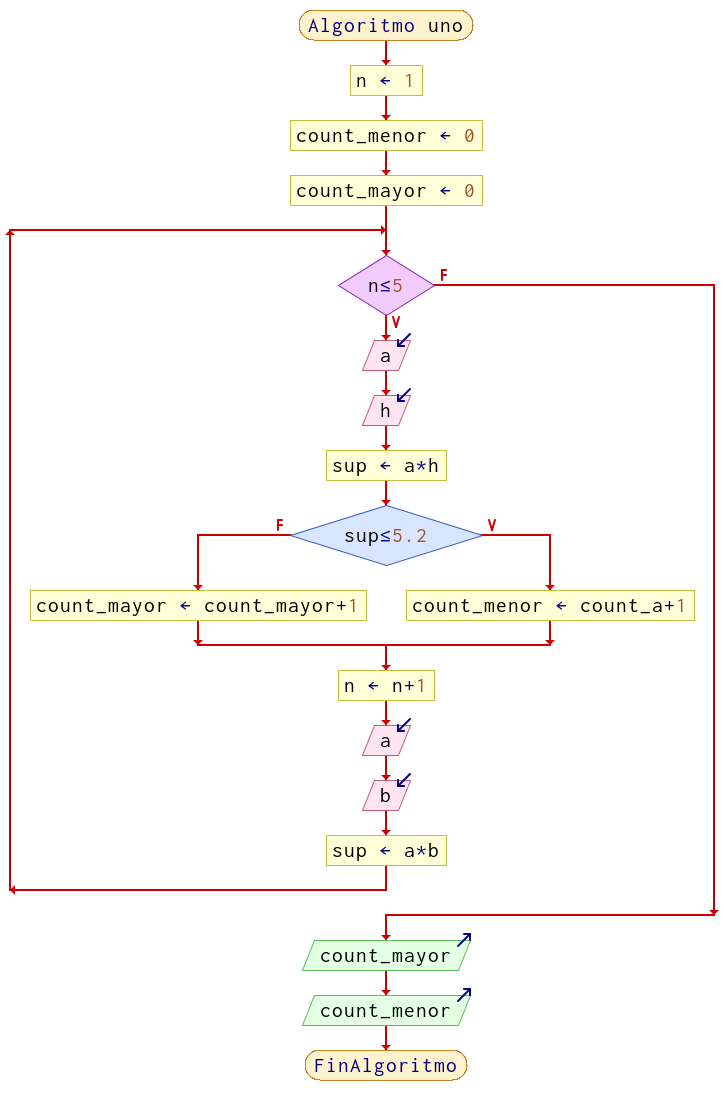
\includegraphics[scale=.3]{imagenes/examen1/1.png}
	\end{center}

    %----------c)
    \item \textbf{Prueba de escritorio.}\\
	\begin{center}
	    \begin{tabular}{c|c|c|c|c|c}
		$a$ & $h$ & $n$ & $sup$ & $count\_mayor$ & $count\_menor$\\
		\hline
		\cancel{1}&\cancel{1}&\cancel{1}&\cancel{1}&&\cancel{1}\\
		\cancel{1}&\cancel{2}&\cancel{2}&\cancel{2}&&\cancel{2}\\
		\cancel{2}&\cancel{2}&\cancel{3}&\cancel{4}&&3\\
		\cancel{2}&\cancel{3}&\cancel{4}&\cancel{6}&\cancel{1}&\\
		3&3&5&9&2&\\
	    \end{tabular}
	\end{center}
	\vspace{1cm}
    
    %----------d)
    \item \textbf{Código fuente.}\\ 
	
	\lstinputlisting[language=Python]{python/examen1/1.py}
	\vspace{1cm}
    
    %----------e)
    \item \textbf{Prueba de la ejecución del programa}.\\
	\begin{center}
	    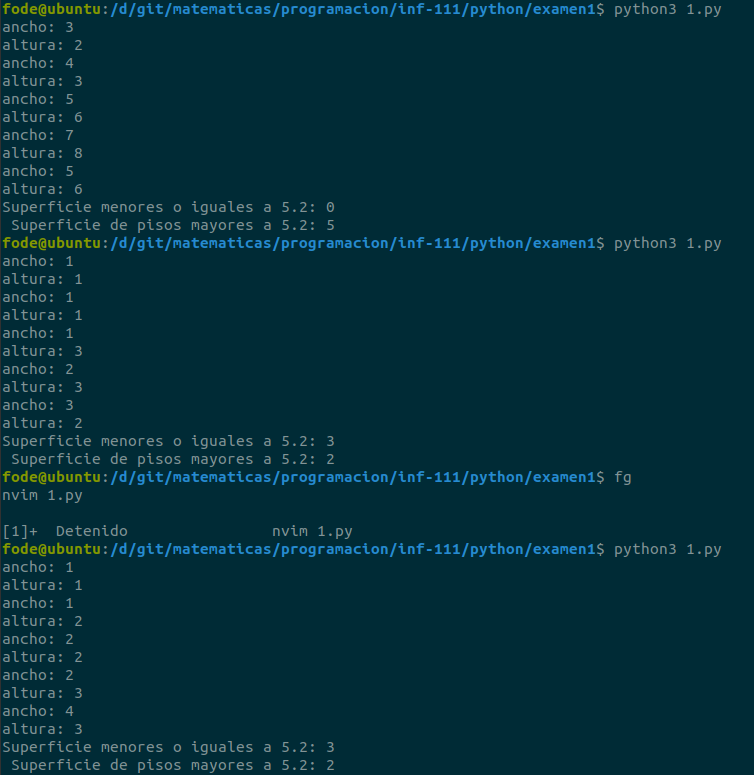
\includegraphics[scale=.35]{imagenes/examen1/1pe.png}
	\end{center}

\end{enumerate}

\newpage

%--------------------2.
\item 
\begin{enumerate}[\bfseries a)]
    
    %----------a)
    \item \textbf{Análisis del problema.}\\\\
	Sean $nc$ el número de cabezas, $np$ el número de patas, $x$ el número de palomas y $nc-x$ el número de conejos, luego sabiendo que cada conejo tienen 4 patas y cada paloma 2 patas, entonces el número de patas de palomas será $2x$ y el número de patas de conejos será $4(nc-x)$, por lo tanto, la ecuación vendrá dada por:
	$$2x+4(nc-x)=np$$
	de donde el número de patas de paloma se conformará por la fórmula:
	$$x = \dfrac{4nc-np}{2}$$
	Por último,  $nc-x$ será el número de conejos.\\\\ 

    %----------b)
    \item \textbf{Diagrama de flujo.}\\
	\begin{center}
	    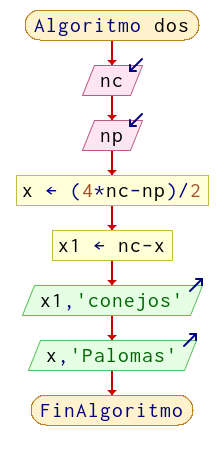
\includegraphics[scale=.5]{imagenes/examen1/dos.png}
	\end{center}

    %----------c)
    \item \textbf{Prueba de escritorio.}\\
	\begin{center}
	    \begin{tabular}{c|c|c|c}
		nc&np&x&x1\\
		\hline
		4&16&0&4\\
		10&40&0&10\\
	    \end{tabular}
	\end{center}
	\vspace{1cm}
    
\end{enumerate}

\newpage


%--------------------3.
\item 
    
    %----------d)
     \textbf{Código fuente.}\\ 
	
	\lstinputlisting[language=Python]{python/examen1/preg.py}
	\vspace{1cm}
    
    %----------e)
     \textbf{Prueba de la ejecución del programa}.\\
	\begin{center}
	    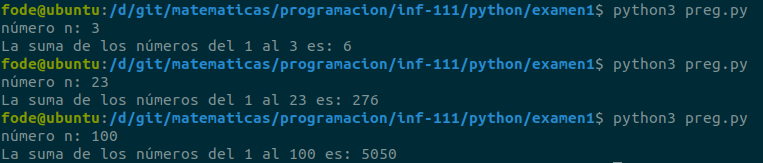
\includegraphics[scale=.5]{imagenes/examen1/preg.png}
	\end{center}
	\vspace{2cm}

%--------------------4.
    \item  
    
    %----------d)
     \textbf{Código fuente.}\\ 
	
	\lstinputlisting[language=Python]{python/examen1/preg2.py}
	\vspace{1cm}
    
    %----------e)
     \textbf{Prueba de la ejecución del programa}.\\
	\begin{center}
	    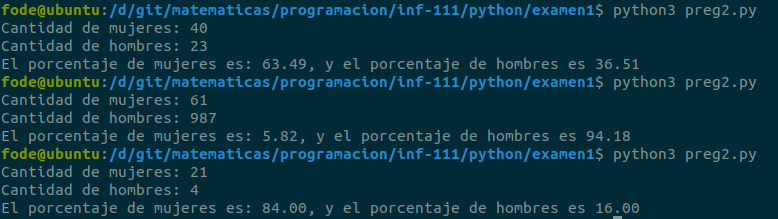
\includegraphics[scale=.5]{imagenes/examen1/preg2.png}
	\end{center}

\end{enumerate}

\newpage
